\chapter{Background}

\section{TF-IDF}

Term Frequency – Inverse Document Frequency is a classic way of guesstimating the importance of a term in a document and corpus. TF-IDF, as the name suggests, is comprised of two parts, term frequency and inverse document frequency: 
\begin{itemize}
    \item \textit{Term Frequency} gives the number of times a term occurs in a document. For example, consider the term "tiger", so term frequency is the number of times "tiger" appears in the article.
    \item \textit{Inverse Document Frequency}: Document frequency is the number of documents a particular term appears in. And so Inverse Document frequency defines the speciality of a term to the corpus or rarity of the term. This is calculated by the log of document count divided by document frequency, that is the number of documents a term occurs in. This reduces the value of most commonly occurring terms such as articles, pronouns, etc. and increases the value for rare occurring terms. It works by determining the relative frequency of words in a certain document compared to the inverse frequency of the occurrence of that word in the entire corpus. It can also be considered to normalize the term weight scores of a term. For example, the term "tiger", does it appear in just 1-2 documents (rare) or almost all documents (common). 
\end{itemize}
This calculation devises the relevance of the particular word in a given document. With this approach, the words that occur more commonly such as articles (a, an, the), pronouns, etc. will have lower relevance score than the terms that are rare or fairly used in a smaller group of documents. In other words, TF-IDF can also be thought of as computing the relative concentration of a term in the corpus. Let's say, the term "tiger" is quite common in a corpus, so the TF-IDF score will be low. But is rare in another corpus, then the TF-IDF score will be high. 
Another important aspect to look at it is the corpus length. For instance, if "tiger" occurs just twice in the 1000 page list, then it probably does not say much about the tiger. However, if "tiger" appears twice in a 54 character tweet, then probably the tweet says a lot about the "tiger".

Most of the search frameworks add certain other parameters along with TF-IDF for relevance score calculations. One such parameter is "fieldNorms", used in Apache Lucene and Elasticsearch. This factor gives substantial preference to shorter documents compared to longer ones. As shown in the "tiger" in the tweet example. The intuition is that the term is highly concentrated in a shorter document, thus the shorter document is more apt to be about the searched term and hence the high importance. However, the base procedure remains the same. For a given document corpus $D$ with size $N$, a term $w$, and an individual document $d \epsilon D$, term weight is calculated as:
\begin{equation} \label{eq:2.1}
        wt_{w,d} = tf_{w,d}*log(\frac{N}{df_{w,d}})   
\end{equation}  

where $tf_{w,d}$ is the number of times term $w$ occurs in a document $d$, and  $df_{w,d}$ is the number of documents in which $w$ appears in $D$.

Now assume that $N \mathtt{\sim} df_{w,d}$ that is, the size of the corpus is almost equal to the number of documents $w$ appears in $D$. Then the value of $log(1+\frac{N}{df_{w,d}})$ will be relatively very small, but still positive. 
If  $ 1 < log(1+\frac{N}{df_{w,d}})) < c $ for some very small constant $c$, then will $wt_{w,d}$ be smaller than  $tf_{w,d}$. This implies that $w$ is relatively common over the entire corpus but still holds some importance throughout $D$ \cite{RN15}.  For instance, the use of words like ‘United’ in United States documents would occur very frequently. Similarly, the articles, prepositions, and pronouns are the most commonly occurring words in any document. These terms do not even hold much relevance in a query, and thus receive a low TF-IDF score, making them negligible in the relevance scoring. 
Considering the converse scenario where $tf_{w,d}$ is relatively large and  $df_{w,D}$ is small. Then the value of $log(1+\frac{N}{df_{w,D}})$  would be large and consequently $wt_{w,d}$ will have a large value. This occurs for rare usage of terms or terms used in a smaller group of documents. If such a term occurs in our search query, then it will be weighed higher and make the document more relevant to the user \cite{RN15}.  

\section{BM25}

Okapi BM25 or more commonly called as BM25(where BM stands for Best Matching) is also one of the standard ranking and term weighting methodology used to determine the relevance of a document for a given search term or query. BM25 stands for "Best Match 25" and its the $25^{th}$ iteration of tuning the relevance calculation \cite{doug2015bm25}. This is based on the probabilistic retrieval framework developed by Robertson, Jones, and others in 1970-80s \cite{robertson2009probabilistic}. The probabilistic model tosses relevance as a probability problem and reflects the probability that a user will find the result relevant to the query.

BM25 is based on the bag of words retrieval model \cite{robertson2009probabilistic}. Similar to TF-IDF, this model is also based on the spatial frequency distribution of terms. BM25 ranks documents based on terms appearing in each document and not on the proximity in the document \cite{Amati2009}. 
The BM25 formula for a term weight is also based on a TF-IDF weighting scheme but with variations in the way TF and IDF terms are calculated. The formula for term weight in BM25 is given as:

\begin{equation}
    wt_{w,d} = \sum_{i}^{n}IDF(q_{i}) * \frac{f(q_{i},D)*(k1+1)}{f(q_{i},D)+k1*(1-b+b*\frac{fieldLen}{avgFieldLen})}
\end{equation}
where,
\begin{itemize}
    \item $q_{i}$ represents the query term q at position i.
    For example, If the search term is "amusement", which is just a single term then $q_{0}$ would be "amusement". If the search term is "amusement park", then ${q_{0}}$ would be "amusement" and $q_{1}$ would be "park". 
    \item $IDF(q_{i})$ represents the inverse document frequency of $q_{i}$. Although the term is called IDF, but there is difference in calculation method. This IDF terms penalizes the term that are more common and reducees thee overall term weight value for the respective term. IDF is calculated as:
    \begin{equation}
        IDF(q_{i}) = \ln(1+\frac{(docCount - f(q_{i}) + 0.5)}{f(q_{i}) + 0.5})
    \end{equation}
    where, $docCount$ is the total number of documents,
    $f(q_{i})$ is the number of documents having the given term $q_{i}$. 
    \begin{figure}
        \centering
        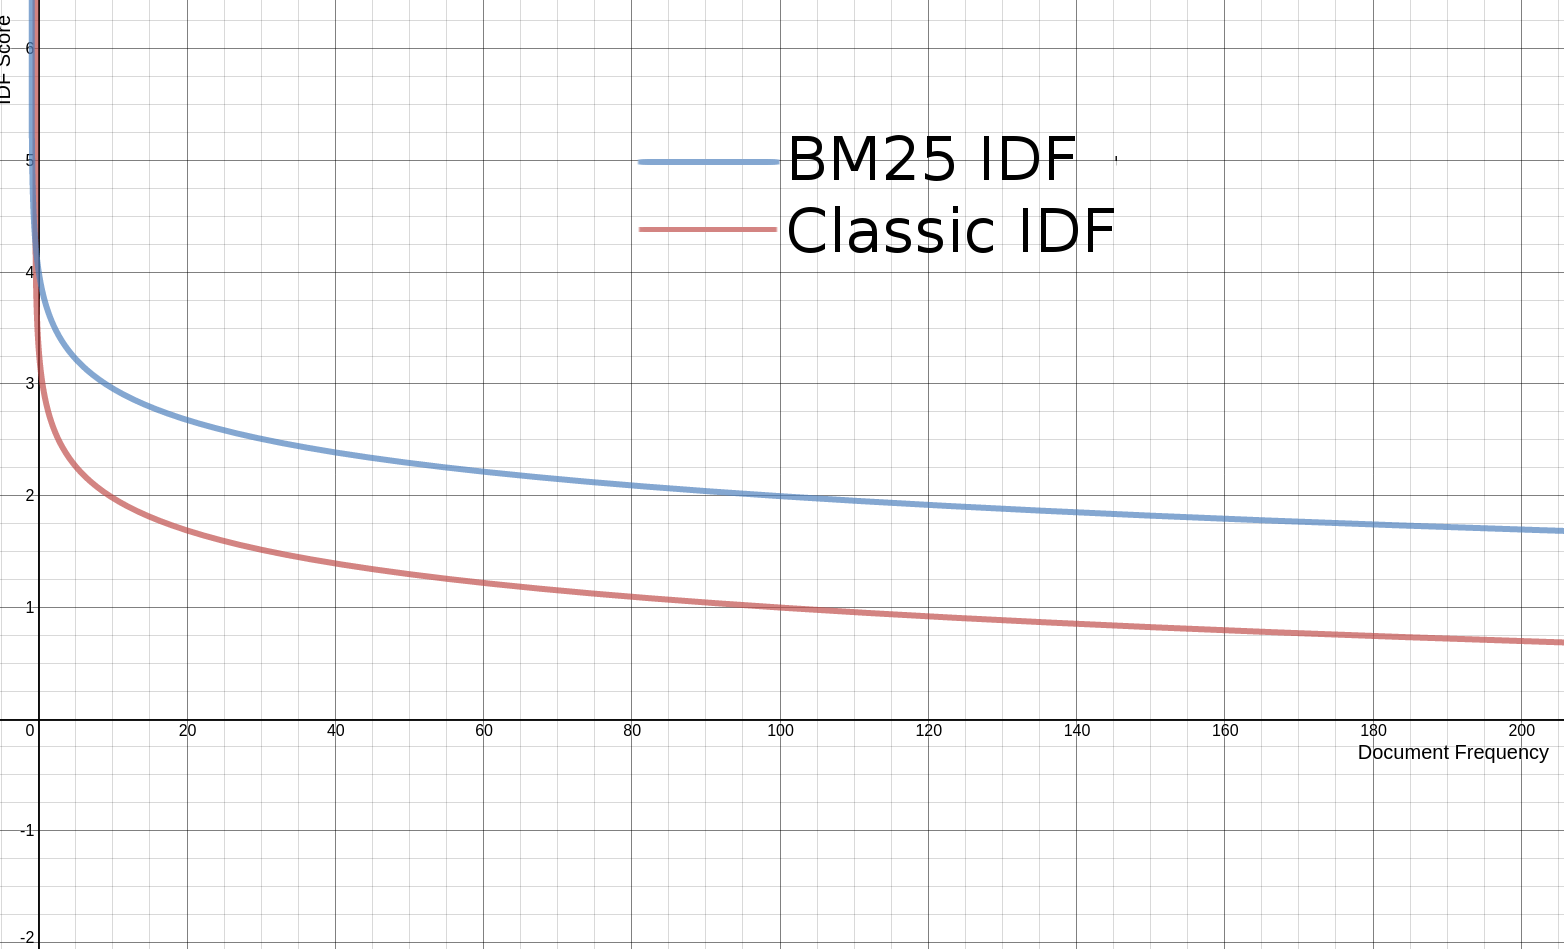
\includegraphics[width=\textwidth]{IDF-comparison-tf-idf-bm25.png}
        \caption{IDF comparison in TF-IDF and BM25}
        \label{fig:IDF-comparison}
    \end{figure}
    Figure \ref{fig:IDF-comparison} shows a comparison of the classic IDF and BM25 IDF. Major change in both the formula is the additional 1. In classic IDF, there are chances of returning a negative values, this is mitigated by use of additional 1 in the log function.
    \item $fieldLen$ denotes the length of present field(or document length) and $avgFieldLen$ denotes the average field length of the entire corpus. 
    $\frac{fieldLen}{avgFieldLen}$ is used in the formula, which calculates the relative length of the present document with respect to the full corpus. The intuition for this is, if the document length is bigger than the average document length, then the denominator becomes large, hence reducing the term weight value. For example, if a term "tiger" appears once in a 200 pages document, then the term might not be significant, however, if the term "tiger" appears twice in a tweet, then it is much relevant about the term.
    \item a constant term $b$, which is multiplied by the field length parameters. If $b$ is large, then the relative length of the document is increased and vice versa. By default, the value of $b$ is 0.75.
    \item $k1$ and $f(q_{i},D)$ are used in both numerator and denominator. Looking at their significance individually,
    \begin{enumerate}
        \item $f(q_{i},D)$ denotes the number of times the term $q_{i}$ appears in a document $D$. This is the same as term frequency used in the TF-IDF formula shown in equation \ref{eq:2.1}.
        The intuition for term frequency is the more number of times a term occurs in a document, more it is relevant to the query.
        \begin{figure}
            \centering
            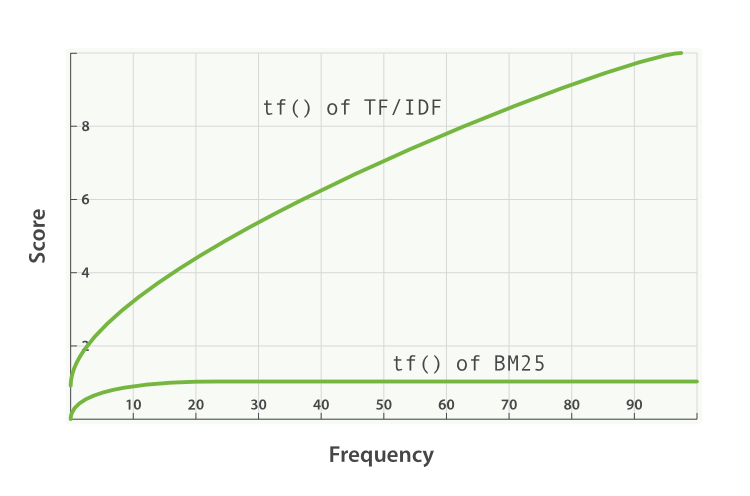
\includegraphics[width=\textwidth]{term_frequency_saturation.png}
            \caption{Term Frequency comparison in TF-IDF and BM25}
            \label{fig:tf-comparison}
        \end{figure}
        \item $k1$ is a constant term to normalize the term frequency $f(q_{i},D)$. This is a new parameter introduced in the BM25 notation. Figure \ref{fig:tf-comparison}  shows the comparison of scores along with term frequency in BM25 and TF-IDF models. This value of k1 can be interpreted as for average length documents, term frequency is approximated to half the actual term frequency of the term. In the figure, we can observe that the score increases rapidly for values where $tf < k1$ and grows gradually when $tf>k1$.
        This k1 value is often set to 1.2. 
        
        
    \end{enumerate}
    
\end{itemize}

\section{Universal Sentence Encoder (USE)}

Universal Sentence Encoder \cite{RN32} is a not specifically a term weighting scheme but a more advanced model used for text embedding into high dimensional vectors and consequently used in tasks such as text classification, semantics, clustering, information retrieval, recommender systems, and other text related tasks.

USE is trained and optimized for more than simple term-based text embedding and works on the sentence level, phrases or small paragraph embedding into a dense vector \cite{RN32}. The USE model is trained on a variety of natural language texts and different data sources to be used in multiple natural language processing tasks. The input is the variable-length English text and the output is a 512 dimension vector. The USE model is trained with a deep averaging network(DAN) encoder \cite{RN32}.
Some of the classic applications of universal sentence encoder are semantic similarity and text classification.
\begin{itemize}
    \item \textbf{Semantic Similarity:} Semantic Similarity shows the level to which two different texts denote the same meaning. This is mainly used to get better results in information retrieval tasks and all related tasks based on understanding natural language. 
    \item \textbf{Text Classification:} Text classification models show better accuracy and efficiency when trained with an enhanced text embedding model such as USE.  Custom binary text classifiers can be trained with the USE model to perform well on the wide variety of classification tasks with a smaller amount of labelled data.
\end{itemize}

The intuition behind USE model is to embed sentence into dense vectors that mark transfer learning tasks to NLP tasks. These models are effectual and result in good performance and accuracy in transfer learning tasks for natural languages. Studies have compared different models implementing word embedding and sentence embedding for trade-offs between accuracy and computational resources. The comparison studies the model complexity, availability of data, and the overall task performance. The comparative analysis shows that the transfer learning along with sentence embedding performs significantly better than the word embedding model and also with a lesser amount of supervised training data availability.

The USE model can be formulated by two methods, first by the use of transformer architecture and the other by the use of deep averaging network(DAN) \cite{RN32}. Both the specified models are implemented using TensorFlow \textbf{[ref]}. The input for these models is English strings and output produced is fixed high dimensional vector representation of the same. This sentence embedding can also be used to compute the sentence level semantic similarity. And experiments show the improved performance of sentence based semantic similarity over the semantic textual similarity. Also, the sentence based models can be trained and modified for improved performance in the gradient-based approaches.

The transformer-based sentence encoding model constructs sentence embeddings using the encoding sub-graph of the transformer architecture \cite{vaswani2017attention}. The sub-graph creates the context-aware representations of every word in a sentence that considers the positioning as well as the meaning of other terms in a sentence. These context-aware representations are then converted into a fixed-length sentence encoding vector by summing the representation of each word position. Next, the encoder takes these string tokens as input and returns a fixed 512-dimensional vector. The encoder is designed as a general-purpose model that can be used in a wide variety of applications. This is achieved by using a single encoding model for multiple tasks. These tasks might include, unsupervised learning for arbitrary running text, a conversational input response task for conversational data, and classification tasks to be trained on the supervised model. 

The second approach model used in USE model is based on deep averaging network(DAN); where the average of input word embedding and bi-grams are passed through a feed-forward deep neural network to produce sentence embedding \cite{iyyer2015deep}. 
Similar to the transformer-based approach, this model takes string tokens as inputs and produces a 512-dimensional sentence embedding.
The training method remains the same as in the transformer-based approach. The major advantage of DAN model is that the compute time is linear for the length of the input sequence. This DAN based also shows significant improvement in text classifications tasks \cite{RN32}.

In classic retrieval method, a common way to convert a text into a numeric vector is by allocating a dimension to every word in the vocabulary. The vector is formulated as the number of times the term occurs in the text corpus. This is referred to as the "bag of words" model, based on just the frequency of terms and not sentence structure \cite{julie2019USE}.

There are certain differences in this traditional approach and text embedding model, they are:
\begin{itemize}
    \item text embedding generates are low dimension vector in the range of 100-1000, whereas the bag of words generates a more sparse matrix with much higher dimensions. This is because embedding model considers semantic context and words with similar meaning will have the same vector representation.
    \item Sentence embedding model considers the order of terms while defining the term vectors. For instance, "tune in" will be given a different vector compared to "in tune". \cite{julie2019USE}
    \item also, sentence embedding model (USE) cannot represent the semantic context for a larger section of text. And can be used only for smaller sentences and phrases.
\end{itemize}

From search and information retrieval perspective, this Universal Sentence Encoder model is incorporated as follows:
\begin{itemize}
    \item all the documents in the corpus are run through pre-trained sentence embedding model to generate its respective dense vector of a given dimension.
    \item similarly, the user query is also run through the same sentence embedding model to produce a numeric vector. And then the similarity between the input query vector and the documents vector is calculated using cosine similarity given in \ref{eq:2.4}
    \begin{equation} \label{eq:2.4}
    \cos \theta = \frac{\sum_{1}^{n} \vec a_{i}b_{i}}{\sqrt{\sum_{1}^{n} \vec a_{i}^2}\sqrt{\sum_{1}^{n} \vec b_{i}^2}}
\end{equation}
\end{itemize}